\chapter{Introduction}
\section{What is Machine Learning ?}

Machine learning is the ability of machines to \tc{learn} from data or past experiences, which come from various sources such as sensors, domain knowledge, experimental runs, etc. Mathematically, it involves making a theoretical function/model $f: X \rightarrow Y$ which predicts outcomes from given inputs, and optimizing it and training it to increase it's prediction accuracy.

\section{Why Machine Learning ?}

We need machine learning in the following cases
\begin{itemize}
  \item When we need to perform tasks that are easy for humans, but complex for computer systems to emulate (eg. distinguishing between a muffin and a Chihuahua)
  \item When we need to perform tasks which are beyond human capabilities, like the analysis of large and complex datasets
\end{itemize}

\begin{center}
  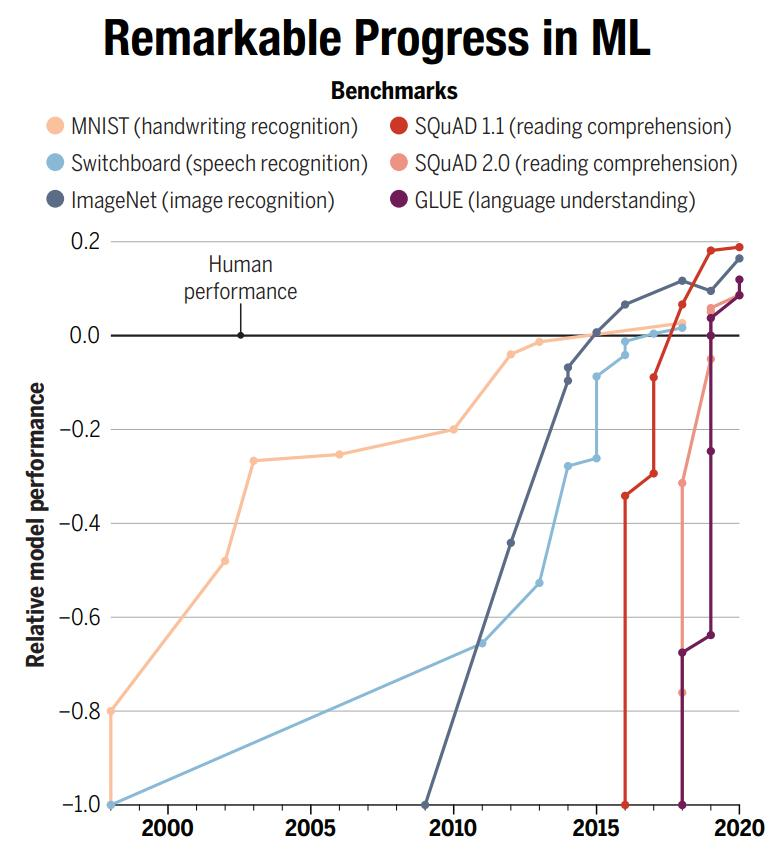
\includegraphics[scale=0.25]{"images/01.jpg"}
\end{center}

Here is a usage histogram for various ML algorithms, which indicates that linear regression and decision trees are very likely to be useful in a machine learning problem.

\begin{center}
  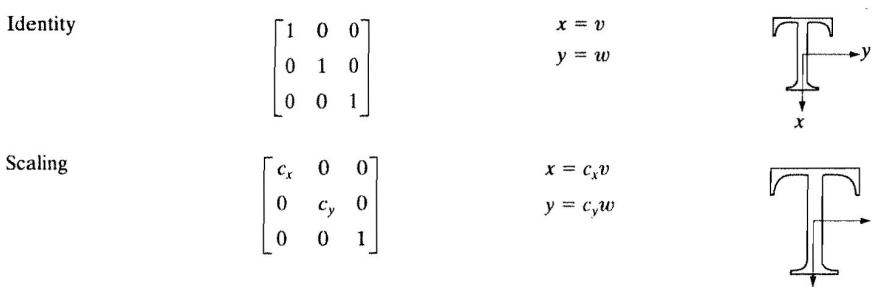
\includegraphics[scale=0.2]{"images/02.png"}
\end{center}

\section{ML Pipeline}
\begin{itemize}
  \item \tc{Data}: Collect data for your problem
        \begin{itemize}
          \item Is the data labelled or unlabelled ?
        \end{itemize}
  \item \tc{Representation}: Choose features that represent your data
        \begin{itemize}
          \item Is the data representation raw, expert-derived or learned ?
        \end{itemize}
  \item \tc{Modeling}: Choose a model for a task
        \begin{itemize}
          \item Should the model be linear/non-linear ? Also, what will be the computational overheads ?
        \end{itemize}
  \item \tc{Training/Learning}: Model will (likely) be parameterized, and these parameters will be learned by training over the data. So, choose a loss function to optimize.
        \begin{itemize}
          \item Which loss function to choose ? And how to best optimise this loss function ?
        \end{itemize}
  \item \tc{Prediction/Inference}: Given a model, assign labels to unseen test instances, then choose an evaluation metric.
        \begin{itemize}
          \item Is the evaluation manual or automatic ?
        \end{itemize}
\end{itemize}

\section{Resources}
Here are some links to find various datasets
\begin{itemize}
  \item \href{https://archive.ics.uci.edu/}{https://archive.ics.uci.edu/}
  \item \href{https://huggingface.co/datasets}{https://huggingface.co/datasets}
  \item \href{http://www.openslr.org/}{http://www.openslr.org/}
\end{itemize}